\documentclass{article}
\usepackage{algorithm}
\usepackage{algpseudocode}
\usepackage{svg}
\usepackage{color}
\usepackage{soul}
\usepackage{xcolor}
\usepackage{amsthm}
\usepackage{float}
\usepackage{sectsty}
\usepackage{amsbsy}
\usepackage{amsthm}
\usepackage{amsmath}
\usepackage{amsfonts}
\usepackage{graphicx}
\usepackage{multirow}
\usepackage{diagbox}
\usepackage{bm}
\usepackage{hhline}
\usepackage{graphicx}
\usepackage{helvet}
\usepackage{enumerate}
\usepackage{amsmath}
\usepackage{amsfonts}
\usepackage{graphicx}
\usepackage{multirow}
\usepackage{subfig}
\usepackage{comment}
\usepackage{mathtools}
\bibliographystyle{plain}

\newtheorem{Algorithm}{Algorithm}[section]
\newtheorem{Definition}{Definition}[section]
\newtheorem{Example}{Example}[section]
\newtheorem{Proposition}{Proposition}[section]
\newtheorem{Lemma}{Lemma}[section]
\newtheorem{Theorem}{Theorem}[section]
\newtheorem{Corollary}{Corollary}[section]
\newtheorem{Proof}{Proof}

\newcommand{\B}{{\mathbb{B}}}
\newcommand{\Z}{{\mathbb{Z}}}
\newcommand{\R}{{\mathbb{R}}}
\newcommand{\Q}{{\mathbb{Q}}}
\newcommand{\N}{{\mathbb{N}}}
\newcommand{\C}{{\mathbb{C}}}
\newcommand{\Zn}{{\mathbb{Z}}_{n}}
\newcommand{\Zp}{{\mathbb{Z}}_{p}}
\newcommand{\F}{{\mathbb{F}}}
\newcommand{\Fbar}{{\overline{\mathbb{F}}}}
\newcommand{\Fq}{{\mathbb{F}}_{q}}
\newcommand{\Jc}{J_c}
\newcommand{\Jz}{J_0}
\newcommand{\Jb}{J_b}
\newcommand{\Jt}{J_2}
\newcommand{\al}{\alpha}
\newcommand{\Joz}{J_1 + J_0}
\newcommand{\Jtz}{J_2 + J_0}
\newcommand{\Fqbar}{{\overline{{\mathbb{F}}_q}}}
\newcommand{\Fkk}{{\mathbb{F}}_{2^k}}
\newcommand{\Zkk}{{\mathbb{Z}}_{2^k}}
\newcommand{\Fkkx}[1][x]{\ensuremath{\mathbb{F}}_{2^k}[#1]\xspace}
\newcommand{\Grobner}{Gr\"{o}bner\xspace}
\newcommand{\bi}{\begin{itemize}}
\newcommand{\ei}{\end{itemize}}

\newcommand{\idealj}{{J = \langle f_1,f_2 \dots, f_s\rangle}}
\newcommand{\idealg}{{J = \langle g_1, \dots, g_t\rangle}}
\newcommand{\vfqj}{{V_{\Fq}(J)}}
\newcommand{\vfqjo}{{V_{\Fq}(J_0)}}
\newcommand{\vfbqj}{{V_{\overline{\Fq}}(J)}}
\newcommand{\vfbqjo}{{V_{\overline{\Fq}}(J_0)}}
\newcommand{\vfbqjjo}{{V_{\overline{\Fq}}(J+J_0)}}
\newcommand{\vfkkj}{{V_{\Fkk}(J)}}
% \newcommand{\v}{\vee}
\newcommand{\acf}{\bar{F}_q}
\newcommand{\Vacf}{V_{\bar{F}_q}}

\sectionfont{\large}

\title{Discussions on recent automatic debugging approaches}
\author{Vikas Rao\\
Department of  Electrical and Computer Eng.\\
University of Utah\\Vikas.k.rao@utah.edu }
\date{}
\begin{document}

\maketitle
\section{Introduction}
The most recent approach which deals with automatic debugging mechanism \cite{farimah:2016} is limited to textbook structure of arithmetic circuits. The coefficient computation in \cite{farimah:2016} borrowed from \cite{maciej:2015:2} is incomplete as it completely relies on the half adder structure and doesn't talk about the ambiguities in coefficient weight calculations when the gate structure differs from the given topology. The approach also fails to arrive at a conclusive solution when the circuit is tweaked with some redundant gates as shown in following sections.

\section{Debug Approach}
In the paper described \cite{farimah:2016}, the approach for automatic debugging of arithmetic circuits is classified into following sub-problems: The first step is to do an equivalence check of the given circuit $C$ against a golden specification $f$ and confirm if at all the circuit is buggy, let us call this step as the remainder generation. Once we have a remainder, we need to identify the test patterns which excite the bug in the design, let us call this step as test generation. Once we identify the test vectors, we need to simulate these vectors to identify all the output bits which differ against the specification outputs (this helps in pruning the potential faulty gate list), let us call this step as fault pruning. The next step is to localize the bug, meaning identify the exact bug location, followed by which we need to find the correct fix such that it conforms to the specification.

We can have either one faulty gate or multiple faulty gates. For simplicity, we shall take a single faulty gate model, i.e.,only one gate in the design has been incorrectly replaced, for example an AND gate replaced with an XOR/OR gate. Based on this model we shall analyze and discuss the debug approach.

\section{Preliminaries}
To perform verification, the algebraic model of the implementation is used, wherein each gate is modeled as a polynomial with integer coefficients, and variables from $\mathbb{Z}_2$ are used. The polynomial computation for the respective gates are as shown below -

\begin{gather*}
z_1 = NOT(a) \rightarrow z_1 = 1-a;\\
z_2 = AND(a,b) \rightarrow z_2 = a\cdot b;\\
z_3 = OR(a,b) \rightarrow z_3= a+b-a\cdot b;\\
z_4 = XOR(a,b) \rightarrow z_4 = a+b-2\cdot a\cdot b;
\end{gather*}

The construction of remainder to match the pattern considers the coefficients carried by the gate inputs as well, which is derived from~\cite{maciej:2015:2} and summarized in figure~\ref{coeff_calc}. Coefficients of the individual gates can be derived similarly. It can be shown that the inputs to an XOR or OR gate must have the same coefficients($c_1=c_2$), otherwise the algebraic equation for this gate will not be satisfied; the output coefficients of these gates will be equal to that of the inputs. While an AND gate can have different coefficients ($c_1,c_2$), the output coefficient will just be the product of its input coefficients($c_1\cdot c_2$).

\begin{figure}[ht]
	\begin{center}
	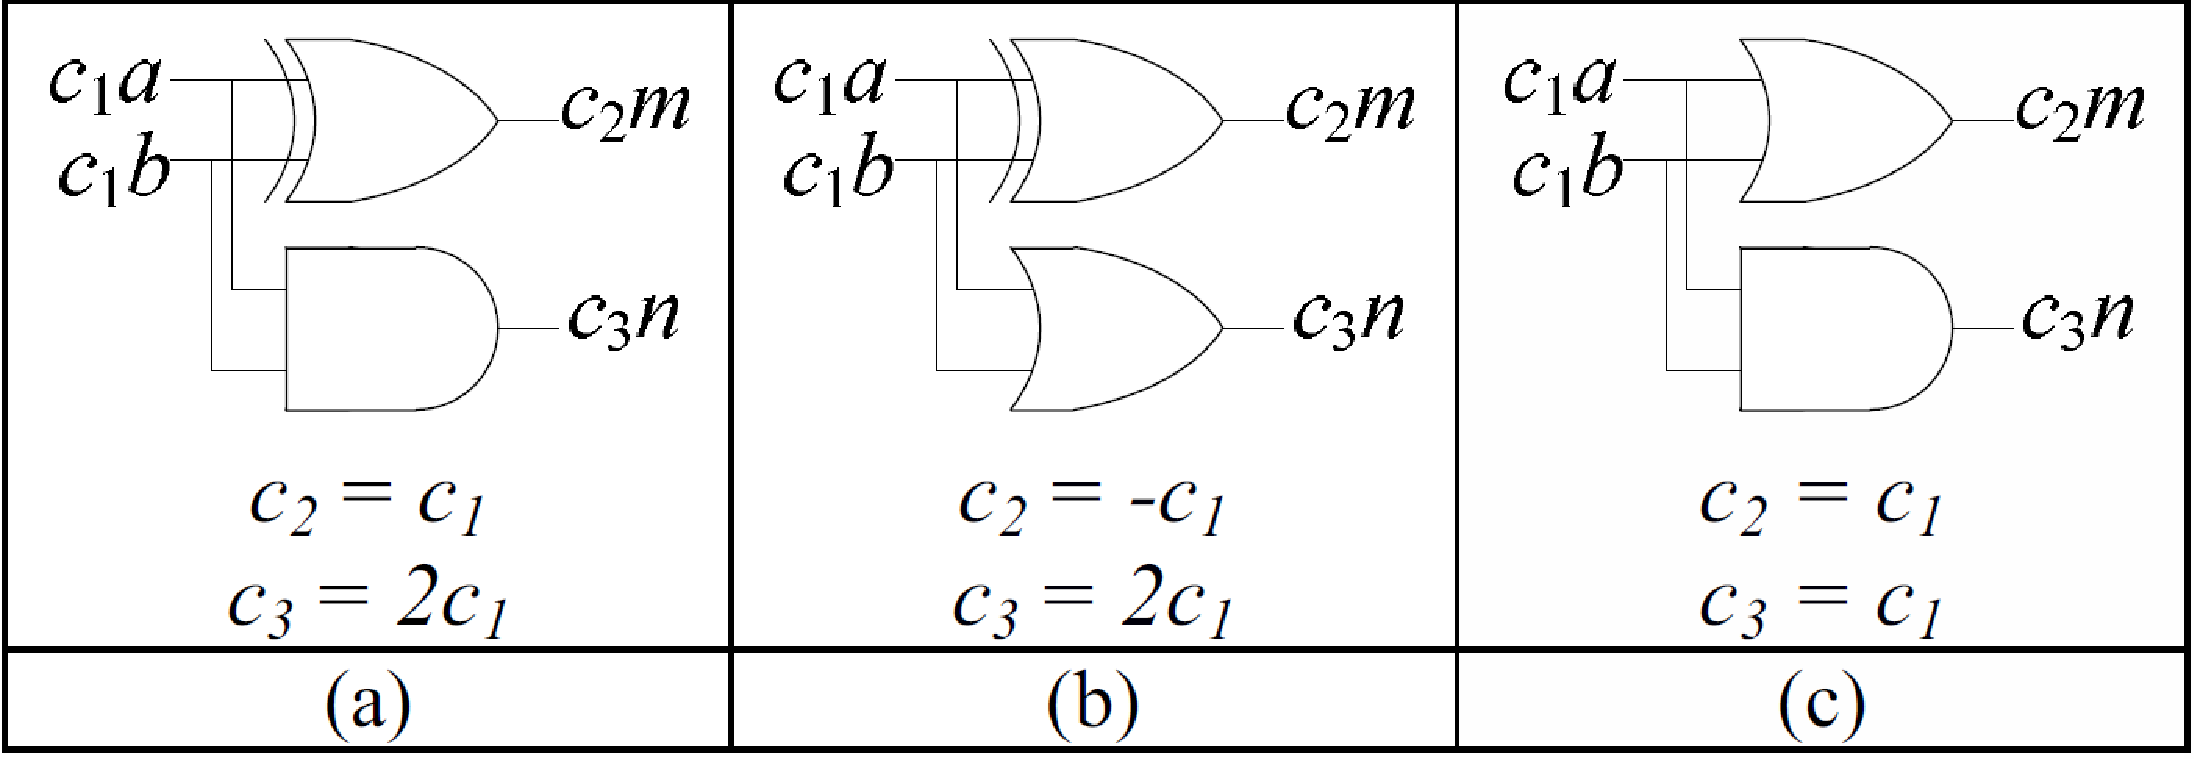
\includegraphics[scale = 0.29]{coeff_calc}
	\end{center}
	\vspace{-4ex}
	\caption{coefficient calculation based on gate structure}
	\label{coeff_calc}
	\vspace{-2ex}
\end{figure}

\subsection{Remainder Generation}
Given specification polynomial $f$ and circuit implementation $C$ as in figure~\ref{int_mul_b}, we need to rewrite $f$ in terms of their gate polynomials derived from the circuit.The approach considers Jinpengs order derived from \cite{lv} wherein they start from the primary outputs, traverse the circuit to the primary inputs, and order the gates according to the their (reverse) topological levels denoted as the Reverse Topological Term Order($RTTO$). 


\begin{figure}[ht]
	\begin{center}
	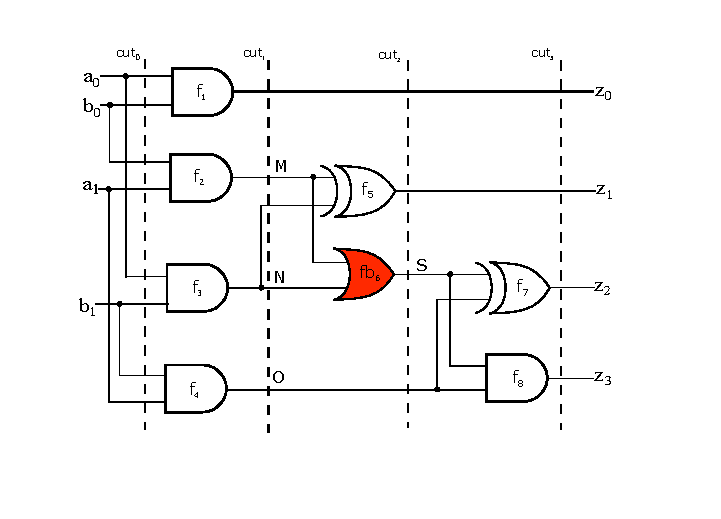
\includegraphics[scale = 0.98]{int_mul_b}
	\end{center}
	\vspace{-4ex}
	\caption{2-bit integer multiplier}
	\label{int_mul_b}
	\vspace{-2ex}
\end{figure}

For the given circuit, RTTO lexicographic order with variable order is given as:
\begin{align*}
\{z_3 > z_2\}>\{z_1> S\}>\{z_0> M> N> O\}>\{a_0> a_1> b_0> b_1\}\\
\end{align*}

The specification rewriting for the circuit in figure~\ref{int_mul_b} is as shown below:

$\text{spec }f: 8.z_3 + 4.z_2 + 2.z_1 + z_0 - 4.a_1.b_1 - 2.a_1.b_0 - 2.a_0.b_1 -a_0.b_0\\$
    $step1: 8.(S.O) + 4.(S+O-2.S.O) + 2.z_1 + z_0 - 4.a_1.b_1 - 2.a_1.b_0 - 2.a_0.b_1 -a_0.b_0\\$
    $step1: 4.S + 4.O + 2.z_1 + z_0 - 4.a_1.b_1 - 2.a_1.b_0 - 2.a_0.b_1 -a_0.b_0\\$
    $step2: 4.(M+N-M.N) + 4.O + 2.(M+N-2.M.N) + z_0 - 4.a_1.b_1 - 2.a_1.b_0 - 2.a_0.b_1 -a_0.b_0\\$
    $step2: 4.M + 4.N + 4.O + 2.M + 2.N -8.M.N + z_0 - 4.a_1.b_1 - 2.a_1.b_0 - 2.a_0.b_1 -a_0.b_0\\$
    $step3: 4.(a_1.b_0) + 4.(a_0.b_1) + 4.(a_1.b_1) + 2.(a_1.b_0) + 2.(a_0.b_1) - 8(a_1.b_0.a_0.b_1) + (a_0.b_0) - 4.a_1.b_1 - 2.a_1.b_0 - 2.a_0.b_1 -a_0.b_0$

\begin{align}
remainder: R = 4.a_1.b_0 + 4.a_0.b_1 - 8.a_0.a_1.b_0.b_1
\end{align}


\subsection{Test Generation}
Once we have a non-zero remainder, we need to identify all the test patterns which excite the bug in the design. The idea is to find assignments to all variables in the remainder such that it makes the decimal value of the remainder non-zero. The approach uses SMT solver by defining Boolean variables and considering signed/unsigned integer values as the total value of the remainder polynomial to identify such assignments.
For example, for the remainder generated in equation(1), $(a_0=0,a_1=1,b_0=1)$ renders the equation to be a non-zero decimal value and hence is one of the test patterns.

\subsection{Gate Pruning}
Once we identify all the input assignments which excite the bug, the next step is to simulate these assignments against the specification polynomial to identify the points of difference in output bits. The idea is to prune the potential faulty gates list to a smaller set. For the given circuit in figure~\ref{int_mul_b}, the test patterns are simulated and compared against the specification polynomial to arrive at the faulty output bits set \{$z_2,z_3$\}. Once we have the affected output bits, the netlist is partitioned to find fanout free cones. The faulty gates in the construction of erroneous output $z_2$ are \{$f_2,f_3,f_4,fb_6,f_7$\}, while for $z_3$ are \{$f_2,f_3,f_4,fb_6,f_8$\}. For a single independent bug, the potential source of error gates are the intersection of these faulty gate lists which gives us the final pruned gate list:$P_g=$\{$f_2,f_3,f_4,fb_6$\}.

\subsection{Bug Localization and Correction}
Now, once we have pruned the gate list, the idea is to characterize the remainder as a pattern by rewriting the remainder in terms of the corresponding gate polynomials. Let's consider the circuit in figure~\ref{int_mul_b} and assume that the AND gate $f_1$ is replaced with an XOR gate. Let us consider the effect of this bug from algebraic point of view: the equivalent algebraic value of the replaced XOR gate is $M=a_0+b_0-2.a_0.b_0$, however the correct implementation with AND gate would have been $M^*=a_0.b_0$. Thus the difference between $M$ and $M^*$ will be ($a_0+b_0-3.a_0.b_0$) and will be observed in the remainder. Similarly for all the possible combinations of erroneous gate replacements, the pattern correlation in remainder will look as described in Table~\ref{correction}.

Once we have the remainder $R$ from equation(1) and the potentially faulty gate list $P_g$, we need to match the remainder pattern against the suspicious patterns in Table~\ref{correction}. The steps to arrive at the remainder pattern matching is as show below: 

\begin{enumerate}
    \item We start from gate $f_2$ and compute $P_1 = -2.a_1-2.b_0+4.a_1.b_0$ and $P_2 = -2.a_1-2.b_0+6.a_1.b_0$. These patterns do not exist in $R$ and hence gate 2 is correct and dictionary will be updated with ($M=2.a_1.b_0$).
    \item Similarly, for gates $f_3$ and $f_4$, the dictionary will be updated with ($N=2.a_0.b_1$) and ($O=4.a_1.b_1$) respectively as their patterns do not match the remainder.
    \item Now, for gate $fb_6$, the patterns can be written as $P_1=4.a_1.b_0+4.a_0.b_1-8.a_1.b_0.a_0.b_1$ and $P_2=4.a_1.b_0.a_0.b_1$
    \item Since, the pattern $P_1$ matches the remainder pattern, the bug is an OR gate and based on the correction mentioned in Table~\ref{correction}, it should be replaced with an AND gate.
\end{enumerate}

\begin{table}[]
\centering
\caption{Remainder pattern correction table}
\label{correction}
\begin{tabular}{|c|c|c|}
\hline
\textbf{Suspicious Gate}&\textbf{Appeared Remainder's Pattern}&\textbf{Solution}\\
\hline
\multirow{2}{*}{AND(a,b)} & $p_1=-a-b+2.a.b$ & $s_1: OR(a,b)$ \\\cline{2-3}
&$p_2=-a-b+3.a.b$ & $s_2: XOR(a,b)$\\
\hline
\multirow{2}{*}{OR(a,b)} & $p_1=a+b-2.a.b$ & $s_1: AND(a,b)$  \\\cline{2-3}
&$p_2=a.b$ & $s_2: XOR(a,b)$\\
\hline
\multirow{2}{*}{XOR(a,b)} & $p_1=a+b-3.a.b$ & $s_1: AND(a,b)$ \\\cline{2-3}
&$p_2=-a.b$ & $s_2: OR(a,b)$\\
\hline
\end{tabular}
\end{table}

\begin{figure}[ht]
	\begin{center}
	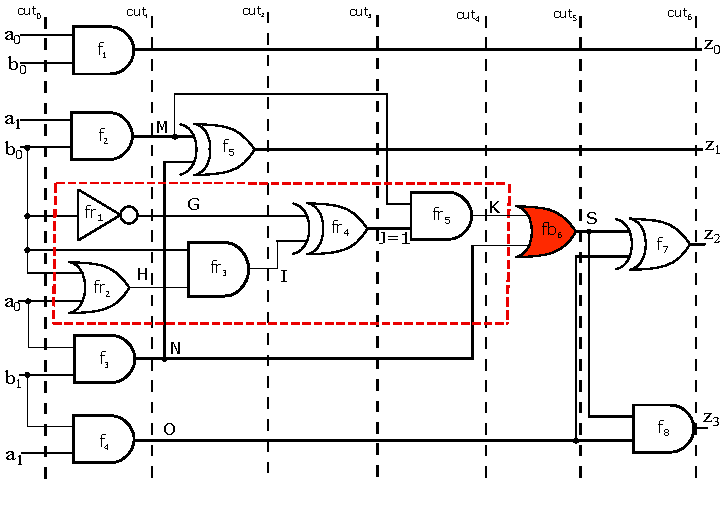
\includegraphics[scale = 0.94]{int_mul_red_b}
	\end{center}
	\vspace{-4ex}
	\caption{2-bit integer multiplier with redundancy}
	\label{int_mul_red_b}
	\vspace{-2ex}
\end{figure}

\section{Counterexample with Redundancy}
Let us consider the circuit in figure~\ref{int_mul_red_b}, wherein we have added a redundant sub-circuit as shown in the dotted red box which evaluates to '$1$'. The final output of redundancy $K$ from $fr_5$ is still $M$, and hence retains the original functionality of the circuit in figure~\ref{int_mul_b}. Let us apply the same procedure on the circuit in figure~\ref{int_mul_red_b} and try to identify the faulty gate.

\subsubsection{Remainder Generation}
Because the redundant circuit evaluates to '$1$', the remainder generated will still be the same and steps are as mentioned before.
\begin{align*}
R: 4.a_1.b_0 + 4.a_0.b_1 - 8.a_0.a_1.b_0.b_1
\end{align*}

\subsubsection{Test Generation}
Since the remainder has the same exact terms and we don't have any new primary inputs introduced for the redundant circuit, the patterns to render a non-zero remainder will also remain the same.

\subsubsection{Gate Pruning}
As the faulty gate is not changed on the redundant circuit design, the affected output bits still remain the same ($z_2,z_3$). Since we have added redundant gates in the design cone, let us reevaluate the gate lists for affected output bits.  
\begin{enumerate}
    \item For $z_2$, the affected gate list is as follows: \\
     \{$f_2,fr_1,fr_2,f_3,f_4,fr_3,fr_4,fr_5,fb_6,f_7$\}, \\
     while for $z_3$:\{$f_2,fr_1,fr_2,f_3,f_4,fr_3,fr_4,fr_5,fb_6,f_8$\}.
    \item The intersection of these lists gives us the potential fault gate list: \\
    \{$f_2,fr_1,fr_2,f_3,f_4,fr_3,fr_4,fr_5,fb_6$\}
\end{enumerate}

\subsubsection{Bug Localization and Correction}
Let us reconstruct the gate polynomials from primary input side for the potential faulty gates to arrive at the matching pattern of the remainder. Let's also record the coefficient values in square brackets when we update the dictionary with the respective gate polynomials.

\begin{enumerate}
    \item Gate $f_2$-AND patterns - $P_1 = -2.a_1-2.b_0+4.a_1.b_0$ and $P_2 = -2.a_1-2.b_0+6.a_1.b_0$. Since it doesn't match the remainder pattern, let's store ($M=a_1.b_0$[coeff - 2])$\rightarrow$($M=2.a_1.b_0$) in dictionary.
    \item Since $fr_1$ patterns don't match, let's store ($G=1-b_0$[coeff - 1])$\rightarrow$($G=1-b_0$) in dictionary.
    \item similarly for $fr_2$, ($H=a_0+b_0-a_0.b_0$[coeff - 1])$\rightarrow$($H=a_0+b_0-a_0.b_0$) is added to dictionary.
    \item similarly for $f_3$, ($N=a_0.b_1$[coeff - 2])$\rightarrow$($N=2.a_0.b_1$) is added to dictionary.
    \item similarly for $f_4$, ($O=a_1.b_1$[coeff - 4])$\rightarrow$($O=4.a_1.b_1$) is added to dictionary.
    \item similarly for $fr_3$, ($I=H.b_0$[coeff - 1])$\rightarrow$($I=(a_0+b_0-a_0.b_0).b_0$[coeff - 1])$\rightarrow$($I=b_0$) is added to dictionary.
    \item similarly for $fr_4$, ($J=G+I-2.G.I$[coeff - 1])$\rightarrow$($J=(1-b_0)+b_0-2.(1-b_0).b_0$[coeff - 1])$\rightarrow$($J=1$) is added to dictionary.
    \item similarly for $fr_5$, ($K=M.J$[coeff - 2])$\rightarrow$($K=a_1.b_0$[coeff - 2])$\rightarrow$($K=2.a_1.b_0$) is added to dictionary.
    \item similarly for last gate $fb_6$, the two patterns are $P_1 = K+N-2.K.N = 2.a_1.b_0+2.a_0.b_1-8.a_0.a_1.b_0.b_1$ and $P_2 = K.N = 4.a_0.a_1.b_0.b_1$.\\
    
    Despite having a close resemblance to remainder $R$, $P_1$ still doesn't have the correct coefficients to match the remainder. Hence,
    ($S=K+N-K.N$[coeff - 4])$\rightarrow$($S=a_1.b_0+a_0.b_1-a_0.a_1.b_0.b_1$[coeff - 4])$\rightarrow$($S=4.a_1.b_0+4.a_0.b_1-4a_0.a_1.b_0.b_1$) is added to dictionary and we have run out of faulty gate list to analyze the remainder pattern matching.
\end{enumerate}

This shows that, when there is redundancy in the circuit, which doesn't alter the function implemented by the circuit, the approach fails to recognize the faulty gate due to the ambiguity in coefficient computation, which results in remainder pattern not being matched.  
\bibliographystyle{ieeetr}
\bibliography{vikas}

\end{document}
